%%%%%%%%%%%%%%%%%%%%%%%%%%%%%%%%%%%%%%%%%%%%%%%%
%
% == AIT CSIM Handout LaTeX Template ==
% == Credit ==
% Assoc. Prof. Matthew N. Dailey
% Computer Science and Information Management
% Asian Insitute of Technology
%
%%%%%%%%%%%%%%%%%%%%%%%%%%%%%%%%%%%%%%%%%%%%%%%%

\documentclass{article}

\usepackage{a4, url, upquote}
\usepackage{graphicx}
\usepackage{hyperref}
\usepackage[cmex10]{amsmath}
\usepackage{amssymb}
\usepackage{placeins}
\usepackage{listings}

\setlength{\textwidth}{6.5in}
\setlength{\textheight}{9in}
\setlength{\oddsidemargin}{0in}
\setlength{\evensidemargin}{0in}
\setlength{\topmargin}{0in}
\setlength{\headheight}{0in}
\setlength{\headsep}{0in}
\setlength{\footskip}{0.5in}

\newcommand{\bheading}[1]{\vspace{10pt} \noindent \textbf{#1}}

\begin{document}

\begin{tabbing}
    \`\=\kill
    \textbf{Workshop:} The WordPress Way
    \` September 11, 2015 \\
    \textbf{Instructor:} Kan Ouivirach ({\tt \small kan@prontomarketing.com})
        and Navarant Pramuksan ({\tt \small oy@prontomarketing.com}) \\
    \textbf{Company:} Pronto Marketing (Research and Develpment Team)
\end{tabbing}

\hrule

\vspace{.25in}

\begin{center}
    \textbf{\Large The WordPress Way: Customizing WordPress Theme and
        Developing WordPress Plugins}
\end{center}

\vspace{.15in}

\noindent \textbf{Introduction:} This workshop is intended for anyone who wants
to learn WordPress and do things the WordPress way. Participants will learn how
to customize a WordPress theme and better understand how WordPress template
hierarchy works. Participants will also learn how to develop a WordPress plugin
to enhance the funtionality of the theme. By the end of this workshop,
participants will be able to develop their own WordPress theme and use
WordPress as a solution to real-world problems.

\section*{Customizing WordPress Theme}

\noindent In this section, we will customize a WordPress theme
``ThirtyFifteen'' and follow the WordPress template hierarchy~[1] to extend a
new template for a new custom post type. Let's get started. \\

\noindent We are going to duplicate the ThirtyFifteen theme and rename it to
TheWordPressWay. Doing this way allows us to keep the originial theme
unmodified and redo this workshop as many times as we want.

\begin{enumerate}
    \item Go to the directory {\tt wp-content/themes/}.
    \item Duplicate the directory {\tt twentyfifteen} and rename it
        to {\tt thewordpressway}.
    \item Open the file {\tt style.css}, remove the current settings in the
        comments, and use these settings below:
        \begin{itemize}
            \item[-] Theme Name: The WordPress Way
            \item[-] Author: {\tt put\_your\_name\_here}
            \item[-] License: MIT
        \end{itemize}
    \item Go to your WordPress site and change the theme to The WordPress Way.
\end{enumerate}

\noindent Right now we should have The WordPress Way theme activated as seen in
Figure~\ref{fig:csim-logo}. Next we are going to make some simple change on a
very simple template. Here the template like 404 page is a good start.

\FloatBarrier

\begin{figure}[t]
    \centering
    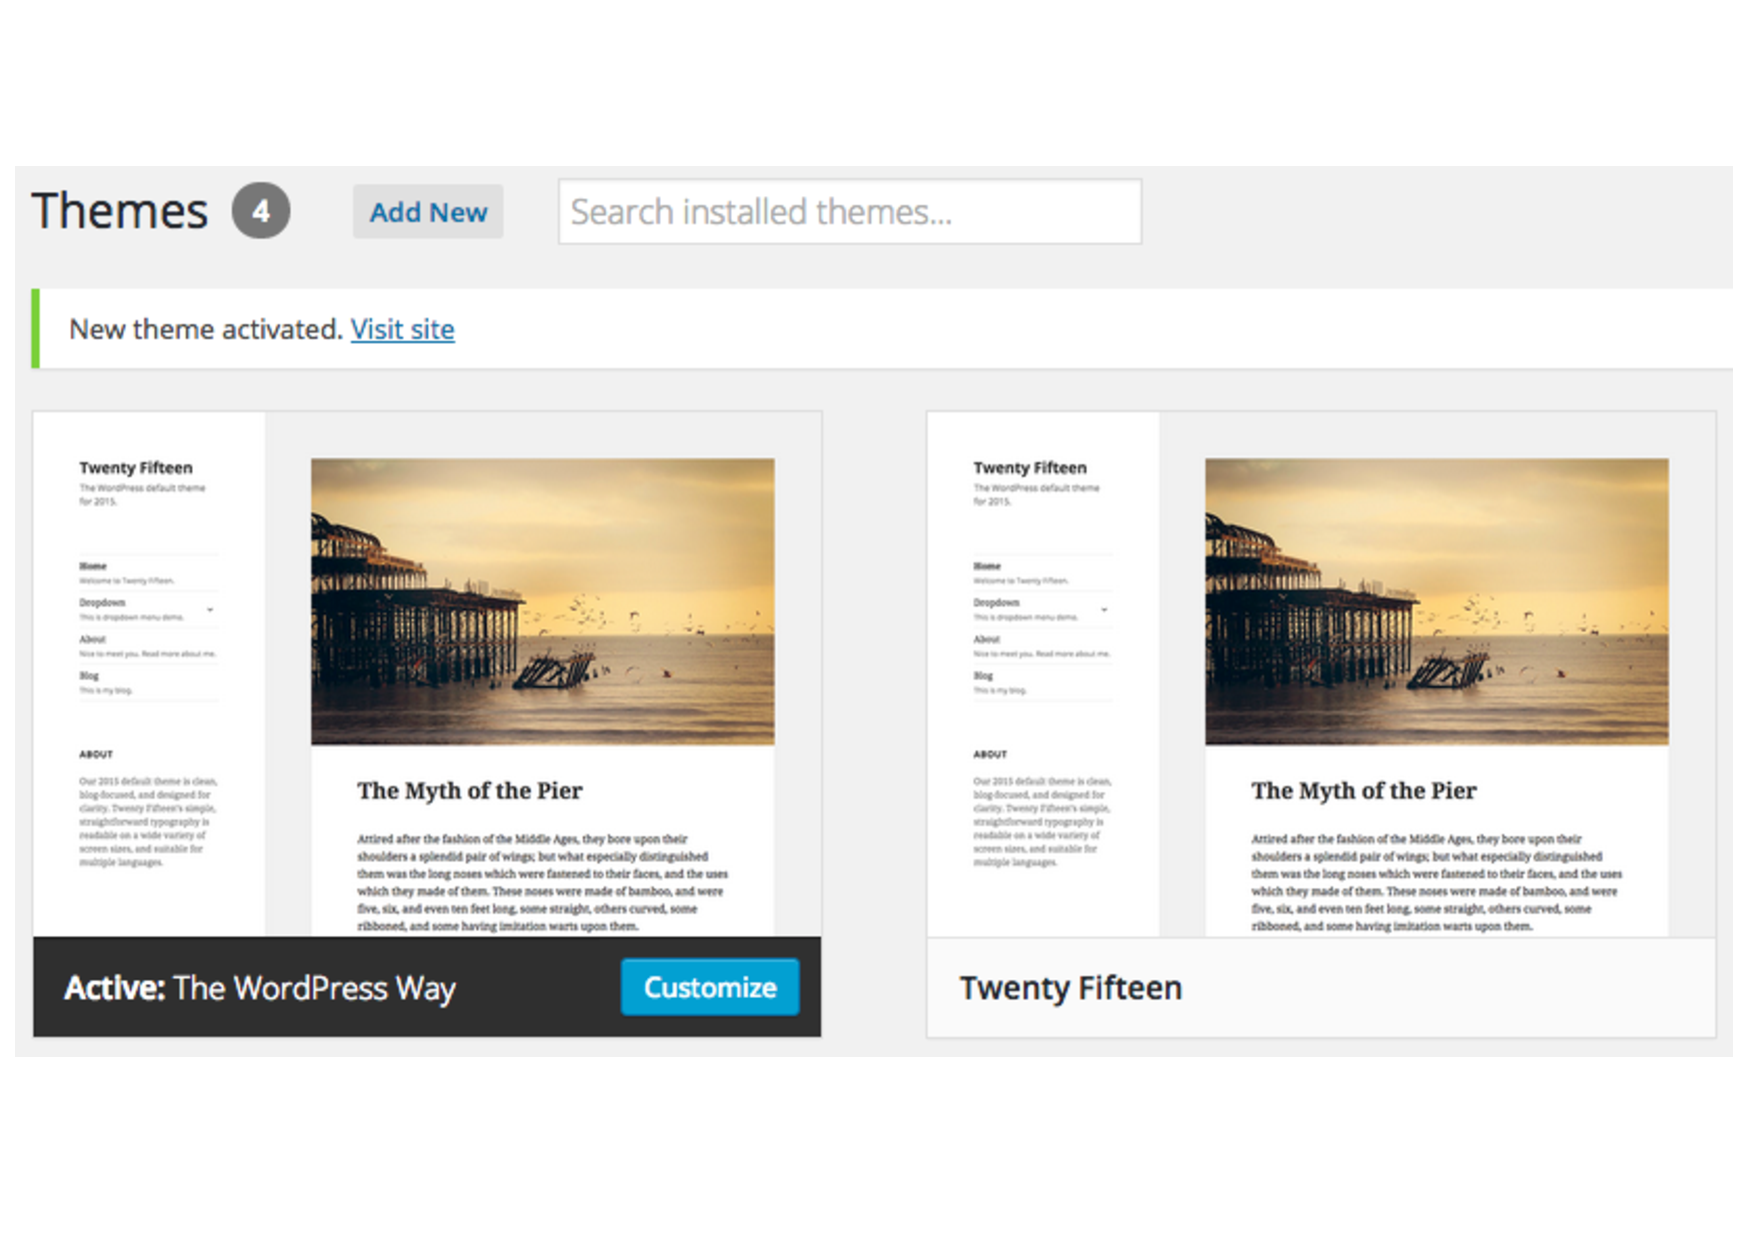
\includegraphics[width=4in]{figures/activating-custom-theme}
    \caption{Activating a Custom Theme}
    \label{fig:activating-custom-theme}
\end{figure}

\begin{enumerate}
    \item Go to your theme directory {\tt wp-content/themes/thewordpressway}.
    \item Open the file {\tt 404.php}.
    \item Let's make it more attractive. Find any image from the Internet and
        put it somewhere on the page. Don't forget to put a credit if the
        image is not yours.
    \item When we access a non-existing page such as
        {\tt http://localhost/?p=99999}, we should see our nice custom
        404 page.
\end{enumerate}

\noindent Your 404 page should look similar to the one shown in
Figure~\ref{fig:custom-404-page}. Below is the code that does that.

\begin{verbatim}
<div id="primary" class="content-area">
  <main id="main" class="site-main" role="main">
    <section class="error-404 not-found">
      <header class="page-header">
        <h1 class="page-title">Oops! Sorry, this page doesn't exist.</h1>
      </header>
      <div class="page-content">
        <p style="text-align: center;">
          <img src="<?php echo get_template_directory_uri(); ?>/images/molodotme.jpg">
        </p>
        <p style="text-align: center;">
          <strong>Credit:</strong> <a href="http://molome.com/" target="_blank">MOLOME</a>
        </p>
        <?php get_search_form(); ?>
      </div>
    </section>
  <main>
</div>
\end{verbatim}

\begin{figure}[t]
    \centering
    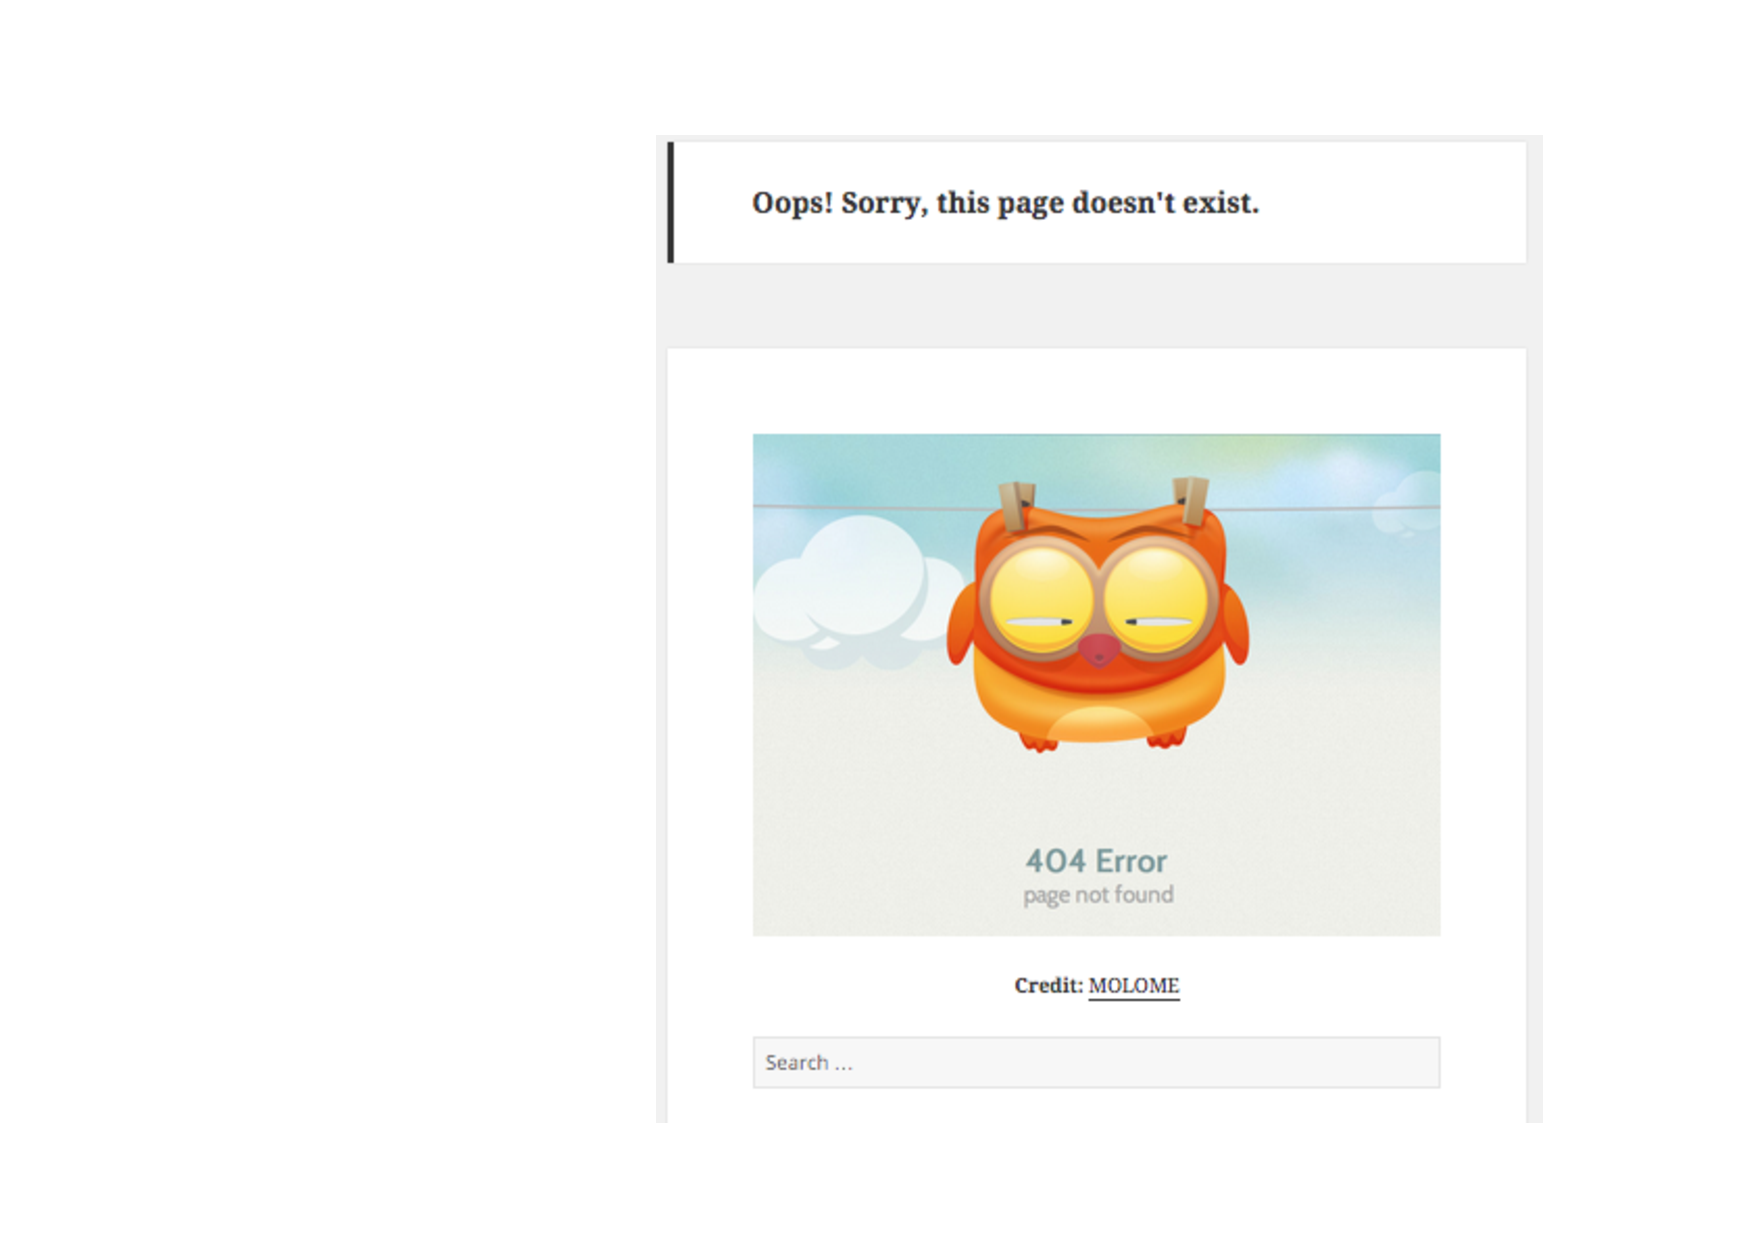
\includegraphics[width=3in]{figures/custom-404-page}
    \caption{Custom 404 Page}
    \label{fig:custom-404-page}
\end{figure}

\noindent Great work! Now you have an experience on customizing the WordPress
template. You can upgrade yourself to the next level, extending the template.
\\

\noindent {\bf Challange:} Let's look at the WordPress template hierarchy for a
minute. Suppose we have our own custom post type and want to create a template
for it. What should we do to accomplish this task? \\

\noindent {\bf Hint:} Read {\tt
http://codex.wordpress.org/Post\_Type\_Templates}.

\section*{Developing WordPress Plugin}

\noindent We will do a simple workshop. Figure~\ref{fig:csim-logo} shows
a logo of CSIM. \\

\noindent Let's follow these steps below.

\begin{enumerate}
    \item Step 1
    \item Step 2
    \item Step 3
\end{enumerate}

\section*{References}

\begin{itemize}
    \item[1] WordPress Template Hierarchy -- \tt{http://wphierarchy.com/}
\end{itemize}

\end{document}
